\scanpage{68}\mspage{67}
\deleted{On a une notion de \unsure{``c|``C|``6}}

Toute partie de $\mathcal F$ (resp $M$) est contenue dans une partie saturée \unsure{minimale} (parmi \unsure{telles|celles} la contenant) qui \deleted{s'appelle \unsure{du|de}} n'est autre que le cosupport du cosupport, et s'appelle aussi son support. Les parties saturées sont celles qui sont égales au support, ou au cosupport, d'une partie. L'application . $\operatorname{cosup}$ \unsure{definit|définit} une \unsure{bij\inserted{e}ction} de l'ens des parties \unsure{saturées|saturée} sur elles $=$, renversant la relation d'inclusion.

On désigne par $\Sigma$ l'ens des \uline{supports} \uline{virtuels}, ou parties saturées
% Figure R1-F1: raised M_0 and its curved oblique insertion leader, without arrowhead.
\figure{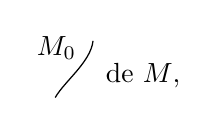
\begin{tikzpicture}[x=1cm,y=1cm]
  \node[anchor=base west] at (0,0) {de $M$,};
  \node[anchor=base east] at (-0.13,0.34) {$\inserted{M_0}$};
  \draw[line width=0.45pt] (-0.52,-0.19) .. controls (-0.40,0.02) and (-0.07,0.26) .. (-0.04,0.53);
\end{tikzpicture}}
où \deleted{\unsure{de}} $\mathcal F_0$ de $M$. \deleted{On \unsure{définit}} \deleted{L'application de cosupport \unsure{d|de}} On \unsure{désidentifie} $\Sigma$ de \deleted{$\unsure{\mathscr P|\mathcal F_2|\mathcal F_0|\mathcal F}$} ses deux 
% Two detached points beneath the word, with no inferred function.
\figure{%
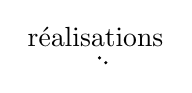
\begin{tikzpicture}[x=1cm,y=1cm]
\node[anchor=base west,inner sep=0] at (0,0) {\unsure{réalisations}};
\fill (0.92,-0.14) circle[radius=0.022cm];
\fill (1.00,-0.20) circle[radius=0.022cm];
\end{tikzpicture}%
}
 (comme \unsure{partie|parties} de $\unsure{P|\mathscr P|\mathcal P}(M)$, ou de $\mathscr P(\unsure{\mathcal F|F})$) et on écrit, pour $\sigma\in\Sigma$
\[
M_\sigma\subset M,\qquad\mathcal F_\sigma\subset\unsure{\mathcal F|F}
\]

Dans $\Sigma$, \deleted{pour} la notion de cosupport est une anti\unsure{\deleted{invo}lution|involution|bijection|dualité} d'ens. ordonnés. Dans $\Sigma$, on a des $\mathrm{Inf}$ quelconques (c'est l'intersection des parties de $M$, ou de $\mathcal F$), et des $\mathrm{Sup}$ quelconques (c'est la partie saturée
